\documentclass[14pt]{extbook}
\usepackage{multicol, enumerate, enumitem, hyperref, color, soul, setspace, parskip, fancyhdr} %General Packages
\usepackage{amssymb, amsthm, amsmath, latexsym, units, mathtools} %Math Packages
\everymath{\displaystyle} %All math in Display Style
% Packages with additional options
\usepackage[headsep=0.5cm,headheight=12pt, left=1 in,right= 1 in,top= 1 in,bottom= 1 in]{geometry}
\usepackage[usenames,dvipsnames]{xcolor}
\usepackage{dashrule}  % Package to use the command below to create lines between items
\newcommand{\litem}[1]{\item#1\hspace*{-1cm}\rule{\textwidth}{0.4pt}}
\pagestyle{fancy}
\lhead{Progress Quiz 10}
\chead{}
\rhead{Version B}
\lfoot{5170-5105}
\cfoot{}
\rfoot{Summer C 2021}
\begin{document}

\begin{enumerate}
\litem{
Which of the following equations \textit{could} be of the graph presented below?
\begin{center}
    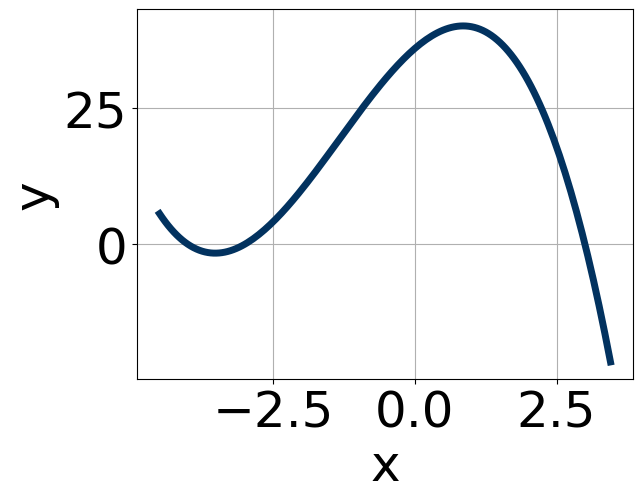
\includegraphics[width=0.5\textwidth]{../Figures/polyGraphToFunctionB.png}
\end{center}
\begin{enumerate}[label=\Alph*.]
\item \( -20(x - 3)^{6} (x + 4)^{11} (x + 3)^{5} \)
\item \( -3(x - 3)^{7} (x + 4)^{9} (x + 3)^{11} \)
\item \( 6(x - 3)^{4} (x + 4)^{11} (x + 3)^{9} \)
\item \( -3(x - 3)^{4} (x + 4)^{8} (x + 3)^{9} \)
\item \( 18(x - 3)^{5} (x + 4)^{5} (x + 3)^{11} \)

\end{enumerate} }
\litem{
Describe the end behavior of the polynomial below.\[ f(x) = 6(x + 4)^{5}(x - 4)^{6}(x - 3)^{4}(x + 3)^{5} \]\begin{enumerate}[label=\Alph*.]
\begin{multicols}{2}\item 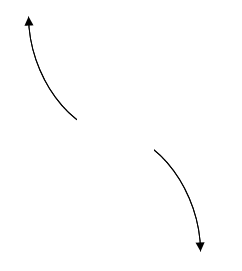
\includegraphics[width = 0.3\textwidth]{../Figures/polyEndBehaviorAB.png}\item 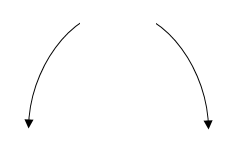
\includegraphics[width = 0.3\textwidth]{../Figures/polyEndBehaviorBB.png}\item 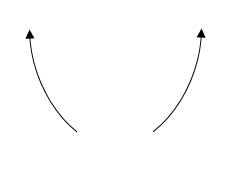
\includegraphics[width = 0.3\textwidth]{../Figures/polyEndBehaviorCB.png}\item 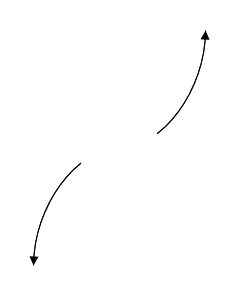
\includegraphics[width = 0.3\textwidth]{../Figures/polyEndBehaviorDB.png}\end{multicols}\item None of the above.
\end{enumerate} }
\litem{
Construct the lowest-degree polynomial given the zeros below. Then, choose the intervals that contain the coefficients of the polynomial in the form $x^3+bx^2+cx+d$.\[ -5 + 5 i \text{ and } -3 \]\begin{enumerate}[label=\Alph*.]
\item \( b \in [-1, 9], c \in [-8, 1], \text{ and } d \in [-15, -11] \)
\item \( b \in [11, 16], c \in [80, 82], \text{ and } d \in [147, 158] \)
\item \( b \in [-1, 9], c \in [7, 11], \text{ and } d \in [11, 19] \)
\item \( b \in [-19, -12], c \in [80, 82], \text{ and } d \in [-158, -146] \)
\item \( \text{None of the above.} \)

\end{enumerate} }
\litem{
Which of the following equations \textit{could} be of the graph presented below?
\begin{center}
    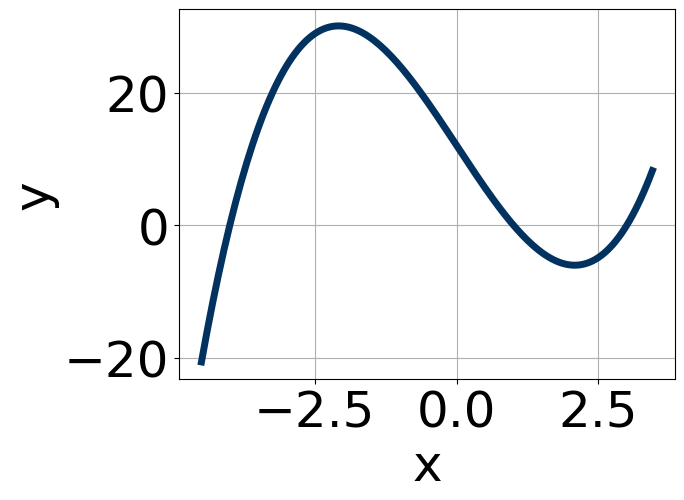
\includegraphics[width=0.5\textwidth]{../Figures/polyGraphToFunctionCopyB.png}
\end{center}
\begin{enumerate}[label=\Alph*.]
\item \( 3(x - 3)^{4} (x + 4)^{8} (x - 1)^{5} \)
\item \( -12(x - 3)^{4} (x + 4)^{5} (x - 1)^{7} \)
\item \( 9(x - 3)^{7} (x + 4)^{11} (x - 1)^{11} \)
\item \( -12(x - 3)^{9} (x + 4)^{11} (x - 1)^{5} \)
\item \( 10(x - 3)^{6} (x + 4)^{11} (x - 1)^{7} \)

\end{enumerate} }
\litem{
Describe the zero behavior of the zero $x = -8$ of the polynomial below.\[ f(x) = 9(x + 2)^{11}(x - 2)^{7}(x + 8)^{7}(x - 8)^{6} \]\begin{enumerate}[label=\Alph*.]
\begin{multicols}{2}\item 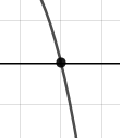
\includegraphics[width = 0.3\textwidth]{../Figures/polyZeroBehaviorCopyAB.png}\item 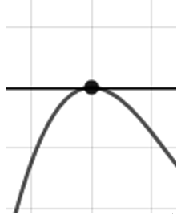
\includegraphics[width = 0.3\textwidth]{../Figures/polyZeroBehaviorCopyBB.png}\item 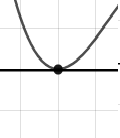
\includegraphics[width = 0.3\textwidth]{../Figures/polyZeroBehaviorCopyCB.png}\item 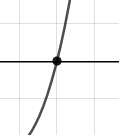
\includegraphics[width = 0.3\textwidth]{../Figures/polyZeroBehaviorCopyDB.png}\end{multicols}\item None of the above.
\end{enumerate} }
\litem{
Construct the lowest-degree polynomial given the zeros below. Then, choose the intervals that contain the coefficients of the polynomial in the form $ax^3+bx^2+cx+d$.\[ \frac{5}{2}, \frac{-1}{3}, \text{ and } \frac{-2}{3} \]\begin{enumerate}[label=\Alph*.]
\item \( a \in [17, 23], b \in [19, 28], c \in [-45, -36], \text{ and } d \in [8, 11] \)
\item \( a \in [17, 23], b \in [-27, -24], c \in [-45, -36], \text{ and } d \in [-17, -9] \)
\item \( a \in [17, 23], b \in [50, 54], c \in [3, 12], \text{ and } d \in [-17, -9] \)
\item \( a \in [17, 23], b \in [58, 75], c \in [44, 53], \text{ and } d \in [8, 11] \)
\item \( a \in [17, 23], b \in [-27, -24], c \in [-45, -36], \text{ and } d \in [8, 11] \)

\end{enumerate} }
\litem{
Construct the lowest-degree polynomial given the zeros below. Then, choose the intervals that contain the coefficients of the polynomial in the form $x^3+bx^2+cx+d$.\[ 4 + 5 i \text{ and } -2 \]\begin{enumerate}[label=\Alph*.]
\item \( b \in [1, 3], c \in [-4.5, -2.7], \text{ and } d \in [-10.1, -9.4] \)
\item \( b \in [1, 3], c \in [-2.53, -1.56], \text{ and } d \in [-8.9, -6.6] \)
\item \( b \in [6, 11], c \in [22.96, 25.33], \text{ and } d \in [-83.9, -75.9] \)
\item \( b \in [-7, -3], c \in [22.96, 25.33], \text{ and } d \in [80.5, 82.2] \)
\item \( \text{None of the above.} \)

\end{enumerate} }
\litem{
Construct the lowest-degree polynomial given the zeros below. Then, choose the intervals that contain the coefficients of the polynomial in the form $ax^3+bx^2+cx+d$.\[ \frac{7}{5}, \frac{-1}{4}, \text{ and } \frac{2}{5} \]\begin{enumerate}[label=\Alph*.]
\item \( a \in [97, 103], b \in [75, 77], c \in [-81, -77], \text{ and } d \in [6, 19] \)
\item \( a \in [97, 103], b \in [-163, -151], c \in [5, 14], \text{ and } d \in [-14, -13] \)
\item \( a \in [97, 103], b \in [-163, -151], c \in [5, 14], \text{ and } d \in [6, 19] \)
\item \( a \in [97, 103], b \in [147, 156], c \in [5, 14], \text{ and } d \in [-14, -13] \)
\item \( a \in [97, 103], b \in [119, 127], c \in [-37, -25], \text{ and } d \in [-14, -13] \)

\end{enumerate} }
\litem{
Describe the zero behavior of the zero $x = -6$ of the polynomial below.\[ f(x) = 9(x - 6)^{5}(x + 6)^{10}(x - 9)^{7}(x + 9)^{11} \]\begin{enumerate}[label=\Alph*.]
\begin{multicols}{2}\item 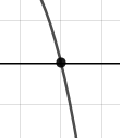
\includegraphics[width = 0.3\textwidth]{../Figures/polyZeroBehaviorAB.png}\item 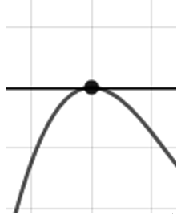
\includegraphics[width = 0.3\textwidth]{../Figures/polyZeroBehaviorBB.png}\item 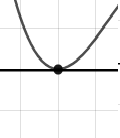
\includegraphics[width = 0.3\textwidth]{../Figures/polyZeroBehaviorCB.png}\item 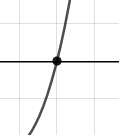
\includegraphics[width = 0.3\textwidth]{../Figures/polyZeroBehaviorDB.png}\end{multicols}\item None of the above.
\end{enumerate} }
\litem{
Describe the end behavior of the polynomial below.\[ f(x) = -8(x - 2)^{4}(x + 2)^{5}(x + 9)^{5}(x - 9)^{6} \]\begin{enumerate}[label=\Alph*.]
\begin{multicols}{2}\item 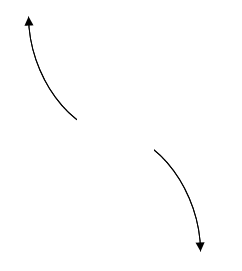
\includegraphics[width = 0.3\textwidth]{../Figures/polyEndBehaviorCopyAB.png}\item 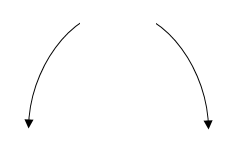
\includegraphics[width = 0.3\textwidth]{../Figures/polyEndBehaviorCopyBB.png}\item 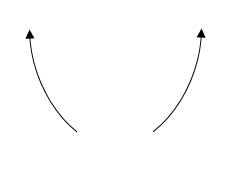
\includegraphics[width = 0.3\textwidth]{../Figures/polyEndBehaviorCopyCB.png}\item 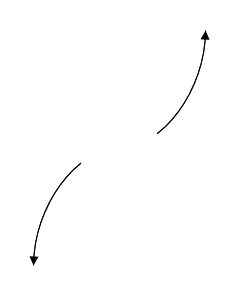
\includegraphics[width = 0.3\textwidth]{../Figures/polyEndBehaviorCopyDB.png}\end{multicols}\item None of the above.
\end{enumerate} }
\end{enumerate}

\end{document}